\documentclass[11pt]{article}
\usepackage{geometry}                % See geometry.pdf to learn the layout options. There are lots.
\geometry{a4paper}                   % ... or a4paper or a5paper or ... 
\usepackage{graphicx}
\usepackage{amssymb}
\usepackage{epstopdf}
\usepackage{tikz} % allows for figures
\usepackage{float} % allows [H] on figure definition
\usepackage{wrapfig}
\usepackage{amsmath} % allows for matrix
\usepackage{subfig}

\DeclareGraphicsRule{.tif}{png}{.png}{`convert #1 `dirname #1`/`basename #1 .tif`.png}

\graphicspath{ {images/} }

% user macros
\newcommand{\R}{\mathbb{R}}
\newcommand{\C}{\mathbb{C}}
\newcommand{\CP}{\hat{\mathbb{C}}}
% end user macros

\title{Equivalent Representations of Circle Packings}
\author{
  Kevin Pratt\\
  \texttt{kevin.pratt@uconn.edu}
  \and
  Connor Riley\\
  \texttt{connor.t.riley@gmail.com}
    \and
  Donald R. Sheehy\\
  \texttt{don.r.sheehy@uconn.edu}
}\date{March 2016}

\begin{document}

\maketitle

\begin{abstract}
  We explore equivalent representations of Circle Packings and the connections between them while presenting an interactive tool for visualizing and experimenting with different circle packing algorithms. 
  The source code can be found at: https://github.com/interl0per/CirclePacking
\end{abstract}

\section{Introduction}

\begin{wrapfigure}{r}{0.4\textwidth}
  \begin{center}
    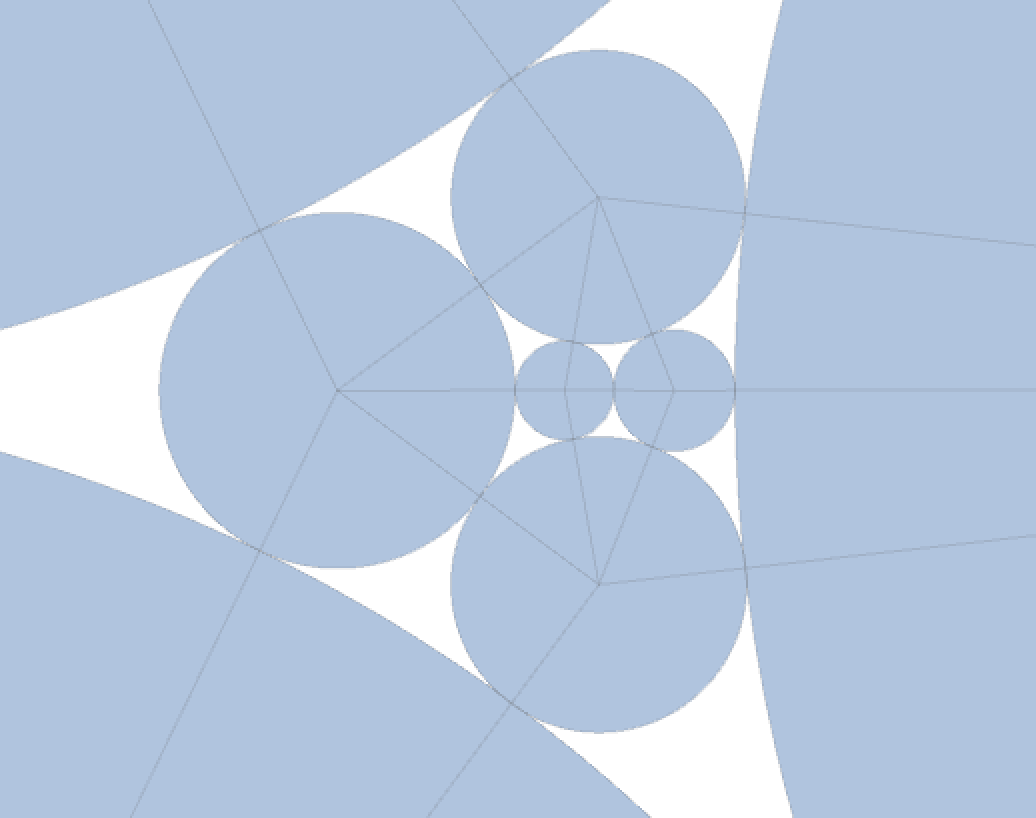
\includegraphics[scale=.18,width=0.45\textwidth]{circlepacking_1}
  \end{center}
  \caption{A unilevant circle packing in a triangle.}
\end{wrapfigure}

The Circle Packing Theorem provides a wonderful link between questions of geometry, topology, combinatorics and complex analysis. Discovered by Paul Koebe and later reintroduced by William Thurston, Circle Packings have become a principle area of study for many mathematicians and geometers. While the formal definition will be introduced later, the intuition for Circle Packings must be developed. A Circle Packing is a configuration of circles with a specified pattern of tangencies \cite{stephenson05introduction}. The Circle Packings most often studied are those that require the interior of the circles to be disjoint, called unilevant packings, this means the circles are non-overlapping \cite{stephenson05introduction}. In this case, a Circle Packing can be thought of as a graph formed by a set of circles which have no overlapping interiors, where each circle kisses its surrounding circles. Two circles kiss or osculate when they intersect at exactly one point. 

Common geometric settings for circle packing are the $euclidean$ $plane$, $the$ $sphere$ and the $hyperbolic$ $plane$. Each pair of circles in a packing forms a tangent pair, and the empty space between each $triple$ forms a $interstice$ \cite{stephenson05introduction}. A $flower$ is the next level of structure, which consists of a central circle and some number of $petal$ circles. The number of petals defines the $degree$ of the central circle. Every circle in a packing has to have a flower, this is called the $local$ $planarity$ condition \cite{stephenson05introduction}. Note that while not all circle packings are unilevant, the ones discussed in this paper and created by the corresponding application will all be unilevant. This means that the interior of all the circles will be mutually disjoint and that the angle sum at each label will be $2\pi$.

The objective of this paper is to explore equivalent representations of Circle Packings and the algorithms they might lead to. To accomplish this goal the theory of Circle Packings will be explored. The other goal is to introduce the reader to the world of Circle Packings, and to do this, basic Geometric principles must be introduced. If you, the reader, are familiar with geometry, then we encourage you to skip the following section.

\section{Introduction to Geometric Figures}
\subsection{Graphs}
A \emph{graph} is an ordered pair $G=(V,E)$ which represents a set of objects where some of these objects are linked. In the denotation $G=(V,E)$, $V$ stands for the vertices or objects, and $E$ stands for the edges or links. Edges in a graph can be directed or undirected, however, we will focus on undirected edges in our application.

  A component or \emph{connected component} of a graph is a subgraph in which any two vertices are connected to each other by a path which is connected to no additional vertices in the supergraph.

  A \emph{self-loop} is when a vertex has an edge connecting it to itself.
  
  A graph with multiple edges is one which has two or more edges connect the same two vertices.

  A graph is \emph{connected} when there is a path between every pair of vertices \cite{mathworld:ConnectedGraphs}. 
  In a connected graph every vertex is reachable. A graph with just one vertex is connected. A graph is said to be \emph{k-connected} if there does not exist a set of k-1 vertices whose removal disconnects the graph. Typically we will work with 3-connected graphs - this means that three vertices would have to be removed to disconnect the graph.
  
  A \emph{simple graph} is an unweighted, undirected graph, containing no loops or multiple edges \cite{mathworld:SimpleGraphs}. 
  A simple graph may either be connected or disconnected.
  
  A \emph{planar graph} is one that can be embedded in the plane. 
  In other words, the graph can be drawn on the plane in such a way that its edges intersect only at their endpoints (no edges cross each other) \cite{mathworld:PlanarGraph}.
  
  A graph $G' = (V',E')$ is a \emph{subgraph} of $G$ ($G' \subseteq G$), if $V' \subseteq V$ and $E' \subseteq E$.
  
  Lastly, an \emph{embedding} of a graph $G$ on a surface $\Sigma$ is a representation of $G$ on $\Sigma$ in which points of $\Sigma$ are associated to vertices and simple arcs are associated to edges in such a way that:
  \begin{itemize}
	\item The endpoints of the arc associated to the edge $e$ are the points associated to the end vertices of $e$.
	\item No arcs include points associated with other vertices.
	\item Two arcs never intersect at a point which is interior to either of the arcs.
  \end{itemize}
  This can be stated mathematically as the following: Given edges $e=(u,v)$, the function mapping the vertices to the plane $ \phi :V \rightarrow \R^2$, and the function mapping the edges to the plane $ \rho_e :[0,1] \rightarrow \R^2$, the embedding $= <\phi, \{\rho_e\} \in E >$

  A \emph{straight-line embedding} is a embedding of a planar graph in which all arcs are straight.


  If $c$ is the number of components in a graph, then a more general form of Euler's formula is:
  \begin{equation} 
	v-e+f= 1 + c
  \end{equation}

Now that we have established the some basic geometric concepts, we can introduce the formal definition of a circle packing.

\section{Circle Packings}
If $\xi$ is an oriented surface with a distance metric then a collection $P = \{c_v\}$ of circles in $\xi$ is said to be a circle packing for a complex $K$ if (1) $P$ has a circle $c_v$ associated with each vertex $v$ of $K$, (2) two circles $c_u$, $c_v$ are tangent whenever $<u,v>$ is an edge of $K$, and (3) three circles $c_u$, $c_v$, $c_w$ form a positively oriented triple in $\xi$ whenever $<u,v,w>$ forms a positively oriented face of $K$ \cite{stephenson05introduction}. 

The \textbf{Discrete Uniformization Theorem}, states, in more general terms, that given any planar graph $G$ with vertex set $V(G) = \{v_1, ... v_n \}$ and edge set $E(G)$, we can find a packing of n (not necessarily congruent) circular discs $C= \{C_1,... C_n\}$ in the plane with the property that $C_i$ and $C_j$ touch each other if and only if $v_i v_j \in E(G)$ for $1 \le i \le n$ \cite{stephenson05introduction}.
By this theorem, circle packings exists for any planar graph, however it is often simpler algorithmically to work with 3-connected, triangulated planar graphs.

The first algorithm in the application is an incremental relaxation algorithm proposed by Stephenson in his book Introduction to Circle Packing. The algorithm begins with a set of tentative radii not necessarily corresponding to a valid packing. In our application, these radii are those input by the user. The algorithm then performs the following steps:
	\begin{enumerate}
		\item Choose an internal vertex $v$ of the input graph.
		\item Calculate the total angle $\theta$ that its $k$ neighboring circles would cover around the circle for $v$, if the neighbors were placed tangent to each other and to the central circle using their tentative radii.
		\item Determine a representative radius $r$ for the neighboring circles, such that $k$ circles of radius $r$ would give the same covering angle $\theta$ as the neighbors of $v$ give.
		\item Set the new radius for $v$ to be the value for which $k$ circle of radius $r$ would give a covering angle of exactly $2\pi$.
	\end{enumerate}
These steps cause the system to converge to a fixed point for which all covering angles are exactly $2\pi$. Once the system has converged, the circles may be placed one at a time, at each step using the positions and radii of two neighboring circles to determine the center of each successive circle.


\begin{figure}%
    \centering
    \subfloat[User input]{{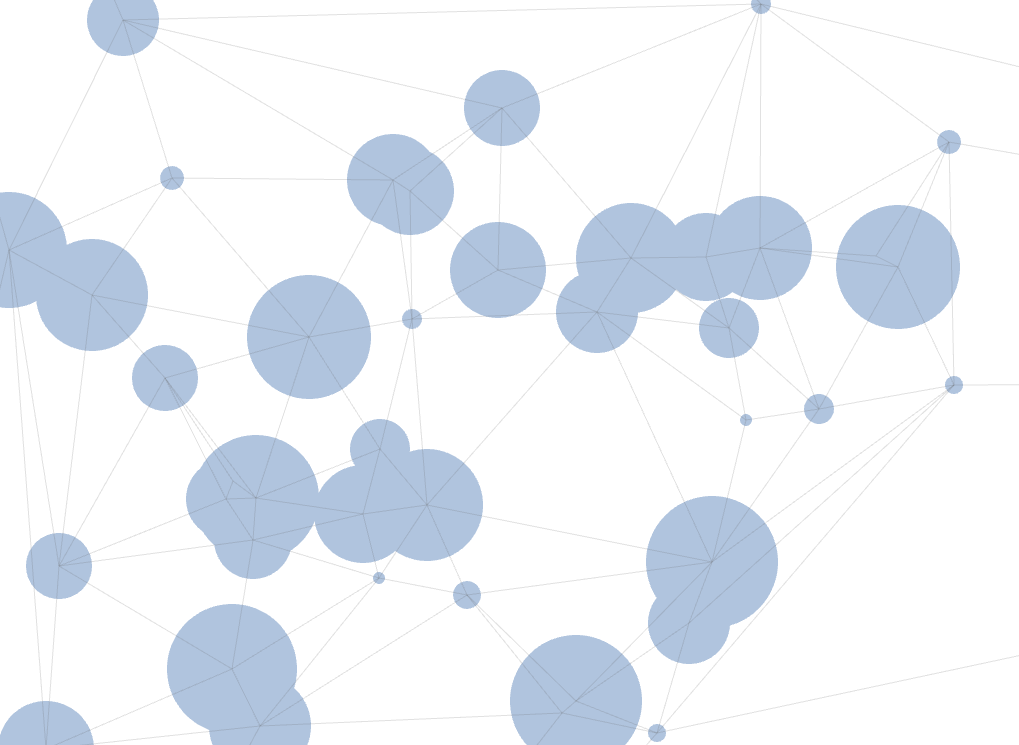
\includegraphics[width=.4\textwidth]{figures/input} }}%
    \qquad
    \subfloat[User input packed]{{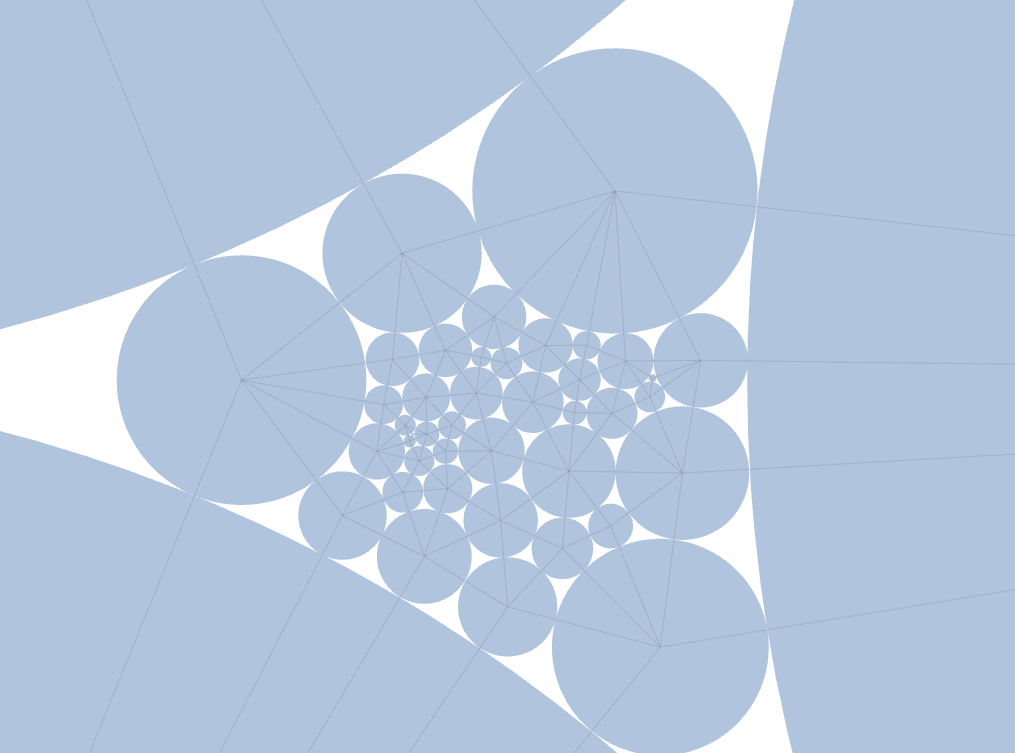
\includegraphics[width=.4\textwidth]{figures/output} }}%
    \caption{Computing a circle packing}%
    \label{fig:inout}%
\end{figure}

\subsection{Delaunay Triangulations}
	A \emph{triangulation}, also referred to as a \emph{maximal planar graph}, is a planar graph in which there is no way to add another edge and have the graph continue to be planar \cite{meshGeneration}. In practice, this means that each face is bounded by three edges - each face is a triangle. This is explained by $Whitney's$ $Theorem$ which concludes that if a graph is planar and 3-connected, all the faces of the graph will be the same shape.

Formally, a triangulation of $S$, a finite set of points in the plane, is a simplicial complex $\tau$ such that $S$ is the set of vertices in $\tau$, and the union of all the simplices in $\tau$ is the convex hull of $S$ \cite{meshGeneration}. Where a simplex is the generalization of the notion of a triangle to arbitrary dimensions.

There are many specific types of triangulations in mathematics, however, we will focus on Delaunay and Weighted Delaunay triangulations.

To explain Delaunay triangulations, some properties of triangles must first be defined. The \emph{circumcircle} of a triangle is the circle which passes through all three of its vertices \cite{mathworld:Circumcenter}. The center of the circumcircle is called the \emph{circumcenter} and the radius is the \emph{circumradius}. The circumcenter can be found by finding the intersection of the \emph{altitudes}, which are formed by drawing a perpendicular line from each vertex to the opposite side of the triangle.
  
A \emph{Delaunay Triangulation} for a set of points $P$ is the triangulation of those points such that no point in $P$ is inside the circumcircle of any other triangle \cite{meshGeneration}. Delaunay triangulations are important largely because in two dimensions they maximize the minimum angle in the triangulation.

\subsubsection{The Edge Flip Algorithm}
An alternate way of describing a Delaunay triangulation is one in which every edge in the triangulation is $locally$ $Delaunay$ \cite{meshGeneration}. For an edge $e$ in the triangulation $\tau$, if $e$ is an edge of fewer than two triangles, then it is automatically locally Delaunay. If $e$ is an edge of exactly two triangles, then $e$ is locally Delaunay if it has an open circumcirlce containing no vertex of either triangle. 

As a result of this property, a trivial algorithm can be formulated that creates a Delaunay triangulation. If $S$ is the point set, this algorithm begins with any triangulation $\tau$ of $S$. Begin with a list of all the edges in the triangulation. Remove an edge from the list, check if the edge is still in the triangulation and if so, if it is locally Delaunay. If the edge is present but not locally Delaunay, flip the edge and add the four surrounding edges to the list of edges to check. This yields an $O(n + k)$ runtime, where in the worst case $k = O(n^2)$ \cite{meshGeneration}.

This leaves one issue, how do we determine whether an edge is locally Delaunay or not. This can be done using the $InCircle$ $test$. Given triangle $abc$ and point $p \in P$ $InCircle(a,b,c,d) \neq 1$ if $abc$ if Delaunay \cite{princeton:CCW}. 
	\begin{equation}
		InCircle(a,b,c,d) = \frac{sign(det
		\begin{bmatrix}
    			a & b & c & d \\
    			\|a\|^2 & \|b\|^2 & \|c\|^2 & \|d\|^2 \\
    			1 & 1 & 1 & 1 \\
		\end{bmatrix} 
		)}{ccw(a,c,b)}
	\end{equation}
	\begin{equation}
		ccw(a,c,b) = det[c-a,b-a] = det
		\begin{bmatrix}
    			a & b & c \\
    			1 & 1 & 1\\
		\end{bmatrix} 
	\end{equation} 
	This equation is simply asking if point $d$ is above of below the plane defined by points $a,b,c$. This is because for any point $a = (x,y)$ the parabolic lifting is defined as $h(x,y) = x^2 + y^2 = \| 
	\begin{bmatrix} 
		x \\
		y \\ 
	\end{bmatrix} 
	\|^2$.
	As a result for any point $a$ the parabolic lifting of $a$, $a'$ is equal to $
	\begin{bmatrix} 
		a \\ 
		\| a \|^2 \\ 
	\end{bmatrix}$. 
	Therefore the lifting of all three points is equal to
	$\begin{bmatrix}
    			a & b & c \\
    			\|a\|^2 & \|b\|^2 & \|c\|^2 \\
	\end{bmatrix}$ 
	is the parabolic lifting of the points $a,b,c$.

An incremental Delaunay algorithm can now be constructed. Given a Delaunay triangulation and a point $p$ to add to the set of points $P$, a new Delaunay triangulation can be created containing point $p$ by first finding the triangle containing point $p$ and then splitting the triangle three ways. This is done by creating edges from point $p$ to each vertex of the triangle. Now that a we have a triangulation the edge flip algorithm is run to make it a Delaunay triangulation. The base case of this algorithm is when you only have three points, in which case, you simply connect the points to create a triangle \cite{meshGeneration}. 

% below this line needs citations
\subsubsection{Voronoi Diagrams}

\begin{wrapfigure}{r}{0.4\textwidth}
  \begin{center}
    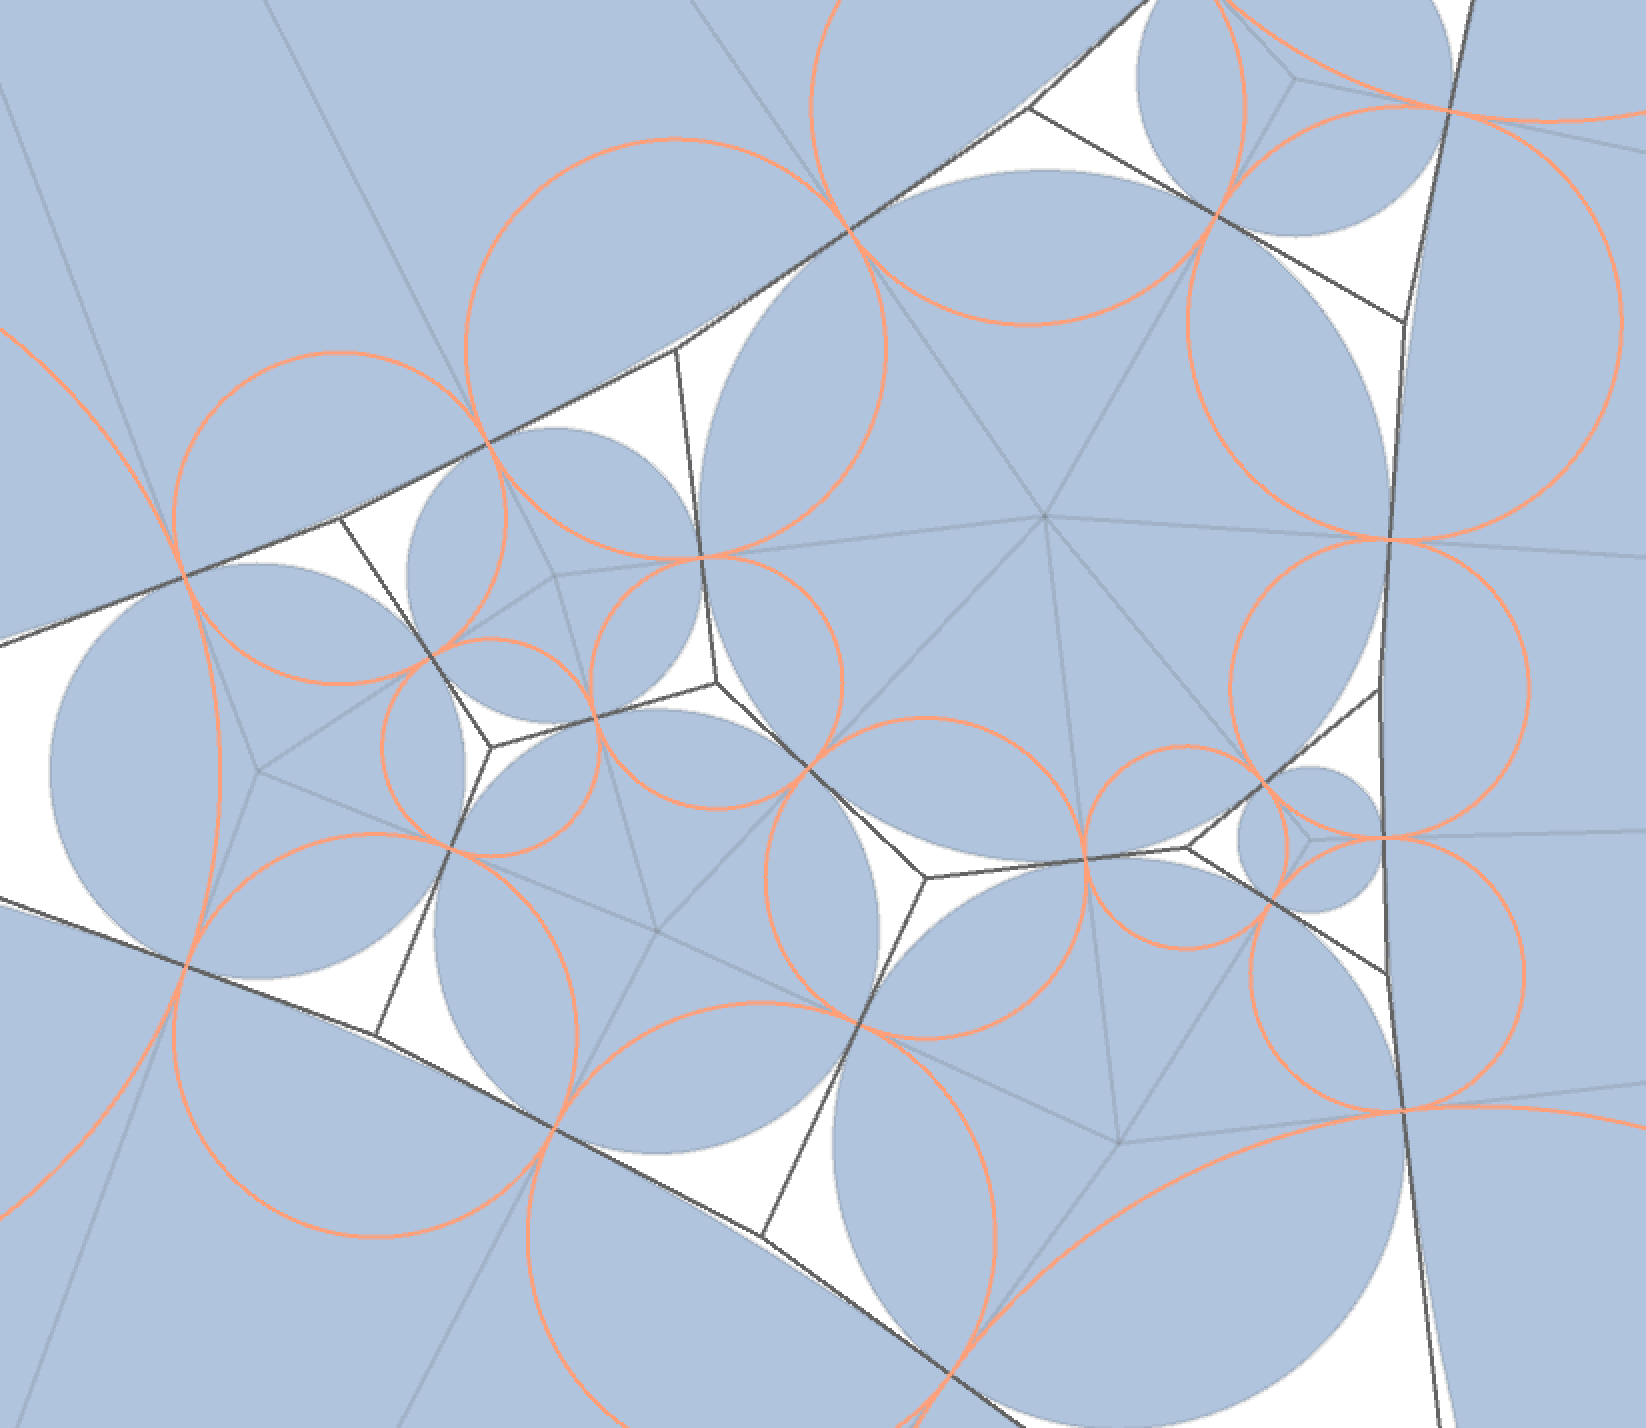
\includegraphics[scale=.18,width=0.45\textwidth]{voronoi}
  \end{center}
  \caption{A circle packing with its dual in red and the Voronoi diagram in black.}
\end{wrapfigure}

Delaunay triangulations are the geometric $dual$ of Voronoi diagrams. A \emph{Voronoi diagram} is the partitioning of a plane into regions based on distance to points in a specific subset of the plane. Formally, the Voronoi diagram of metric space $X$ with a distance function $d$, where $K$ is the set of indices and $P_k, k \in K$ is a tuple of nonempty subsets in the space $X$, is composed of Voronoi cells $C_k$ associated with the site $P_k$. $C_k$ is the set of all points in $X$ whose distance to $P_k$ is not greater than their distance to the other sites $P_j$ \cite{voronoiDiagrams}. 

While Voronoi diagrams can be understood without understanding geometric duals, expanding our understanding of duals will help build the intuition for the connection between the Voronoi diagram and the Delaunay triangulation. This means that the faces, also called 2-cells, of the Voronoi diagram correspond to the points of the Delaunay triangulation. The edges of the Voronoi diagram, also called 1-cells, correspond to the edges, 0-cells, of the Delaunay triangulation and the vertices of the Voronoi diagram correspond to faces of the Delaunay triangulation. The edges of the Voronoi Diagram are orthogonal to the edges of the Delaunay triangulation. These relationships are a result of the fundamental relationships between a dual and primal graph.

In two dimensions, those relationships are as follows: point $p = 
	\begin{bmatrix}
		p_x \\
		p_y \\
	\end{bmatrix} \leftrightarrow $ line $p* = 
	\begin{bmatrix}
		2p_x \\
		-p_y \\
	\end{bmatrix}$ and line $\ell = 
	\begin{bmatrix}
		\ell_n \\
		\ell_b \\
	\end{bmatrix}$ point $\ell* = 
	\begin{bmatrix}
		\frac{1}{2}\ell_n
		-\ell_b
	\end{bmatrix}$. In three dimensions, the relationships undergo similar transformations $point \leftrightarrow plane$, $line \leftrightarrow line$. As a result, lifting the points of a graph from the plane to a 3-dimensional space then taking the dual of those points to obtain hyperplanes and lastly, projecting those planes back onto the original 2-dimensional plane yields a Voronoi diagram and as a result is another way to obtain the Delaunay triangulation.
	
Lastly, just as the Delaunay triangulation is the lower hull of the parabolic lifting, the Voronoi diagram is the upper hull.


% TODO: Add to this subsubsection
\subsubsection{Weighted Delaunay Triangulations}
The weighted Delaunay triangulation is the dual to the so-called power diagram, a Voronoi diagram on the points where the (squared) distance to a circle $c$ with center $p$ and radius $r$ is defined to be $\pi_c(x)^2 := \|x-p\|^2 - r^2$.
  A circle packing representation of a graph realizes the graph as the weighted Delaunay triangulation where the vertices are the centers of the disks and the weights are the radii.

% Need citations end

\section{Embeddings, Liftings and Stress}
From the Discrete Uniformization Theorem we have seen that every planar graph has a Circle Packing. While this is the most general result of this theorem, it can also be said that every 3-connected, triangulated planar graph also has a Circle Packing. Through Tutte's Theorem and the Maxwell Cremona Theorem, we will explore the relationship between embeddings, liftings and stresses and their connection to circle packings.

First, these three terms must be well defined. A \emph{stress} is an assignment of real numbers to edges that may be interpreted as spring constants. By Hook's Law, the magnitude of the force exerted by a spring is the spring constant times its length. A stress is an \emph{equilibrium stress} if for each vertex, the sum of the forces exerted on it by all its incident edges is exactly zero \cite{AresRiboMor}.
Second, a \emph{lifting} (of a planar straight line graph) is an assignment of heights to vertices such that the vertices of each face are coplanar in $\R^3$ (the faces are flat) \cite{WhiteleyHandbook}.
Lastly, an \emph{embedding} of a graph $G$ on a surface $\Sigma$ is a representation of $G$ on $\Sigma$ in which points of $\Sigma$ are associated to vertices and simple arcs, which are images of continuous injective maps [0,1] $\rightarrow \Sigma$, are associated to edges in such a way that:
  \begin{itemize}
	\item The endpoints of the arc associated to the edge $e$ are the points associated to the end vertices of $e$.
	\item No arcs include points associated with other vertices.
	\item Two arcs never intersect at a point which is interior to either of the arcs.
  \end{itemize}
  This can be stated mathematically as the following: Given edges $e=(u,v)$, the function mapping the vertices to the plane $ \phi :V \rightarrow \R^2$, and the function mapping the edges to the plane $ \rho_e :[0,1] \rightarrow \R^2$, the embedding $= <\phi, \{\rho_e\} \in E >$ \cite{mathworld:Embedding}.
 A \emph{straight-line embedding} is a embedding of a planar graph in which all arcs are straight.

This leads us to Tutte's Theroem, which allows us to convert from a simple 3-connected planar graph to an embedding where all the faces are convex. The algorithm to get to this result involves fixing the outer face and assigning arbitrary stresses, in our case of value 1, to each interior edge. Then the equilibrium stress is computed on the interior edges. While the outer face does not have a stress after performing this algorithm, because we have a special case, we can assign the outer face negative stresses to balance out those on the interior and obtain the equilibrium stress. This notion will now be formalized.

\subsection{Tutte's Theroem}
 Given a graph $G=(V,E)$ to each edge $\{i,j\}\in\sigma$ we assign as weight $w_ij\in\R$ also known as a \emph{stress} that represents the elasticity constant of the corresponding rubber band. $w_ij$ must be equivalent to $w_ji$. A negative weight means that the edge is pushing on its two endpoints, whereas a positive weight means that the edge is pulling on the endpoints. 
  
  A \emph{Tutte embedding} or barycentric embedding of a simple 3-connected planar graph is a crossing-free straight-line embedding with the properties that the outer face is a convex polygon and that each interior vertex is at the average (or barycenter) of its neighbor's positions. If the outer polygon is fixed, this condition on the interior vertices determines their position uniquely as the solution to a system of linear equations. Solving the equations geometrically produces a planar embedding. 
  
  Tutte's spring theorem states that this unique solution is always crossing-free, and more strongly that every face of the resulting planar embedding is convex. It is called the spring theorem because such an embedding can be found as the equilibrium position for a system of springs representing the edges of the graph provided the outer face is fixed.
 
 \textbf{Tutte's Theorem} \cite{realizationSpaces}: Let $G = (\{1,...,n\},E)$ be a 3-connected planar graph that has a face $(1,...,k)$ for some $k<n$. Let $p_1,...,p_k$ be the vertices of a convex k-gon. Let $E'$ be the set of interior edges and let $w : E \rightarrow \R^+$ be an assignment of positive weights to the interior edges. Then,
 	\begin{itemize}
		\item There are unique equilibrium positions $p_{k+1}, ...p_n \in \R^2$ for the interior vertices. 
		\item All faces of $G$ are realized as non-overlapping convex polygons.
	\end{itemize}
	
Let $\omega : E \rightarrow \R$ be an assignment of weights to the edges of a graph and let $p:V \rightarrow \R^2$ be an assignment of positions in $\R^2$ for the vertices of $G$. A vertex $v \in V$ is in equilibrium if  $\sum\limits_{\{v,w\} \in E} \omega_{v,w}(p_v - p_w) = 0$

\subsubsection{Proof of Tutte's Theorem}
The following is a summary of a proof by Jurgen Richter-Gebert \cite{realizationSpaces}.

Assume that the positions of the points making up the outer face, points $p_v = (x_v,y_v); v \in \{k+1,...,n\}$, are given. We have to prove that suitable positions $p_v = (x_v,y_v); v \in \{1,...,k\}$ for the interior vertices exist and that these positions are unique. Without loss of generality we may assume that $p_n = (0,0)$. Consider the function
\begin{center}
$E(z) = \frac{1}{2} \sum\limits_{\{v,w\} \in E'} \omega_{v,w}((x_v - x_w)^2 + (y_v - y_w)^2)$ \\
$= \frac{1}{2} \sum\limits_{\{v,w\} \in E'} \omega_{v,w} \|p_v - p_w\|^2$. \\
\end{center}
where $z = (x_1,..x_k, y_1,...y_k)$.
$E$ is a quadratic function that is non-negative everywhere. Assume that one of the points has a coordinate, either $x$ or $y$ with large absolute value. Without loss of generality lets say this coordinate is $x_i$. This implies that $p_i$ is far away from the point $p_n = (0,0)$. Since the graph $G$ is connected, there is a path that connects $p_i$ with $p_n$ and for at least one edge $(v,w)$. In this path the distance $\|p_v - p_w\|$ is large. Since the squared distances are weighted with positive coefficients $E(z)$ is also large. Thus for sufficiently large $\alpha > 0, \|z\| > \alpha$ implies $E(z) > E(0)$. This means that $E$ must be strictly convex and thus takes its unique minimum on $\{z | |z| < \alpha \}$. The assertion follows from the observation that the condition for a critical point $(\triangledown E = 0)$ of $E$ is
\begin{center}
$\frac{\delta E}{\delta x_i} = \sum\limits_{\{v,w\} \in E'} \omega_{v,w}(x_v - x_w) = 0$ and $\frac{\delta E}{\delta x_i} = \sum\limits_{\{v,w\} \in E'} \omega_{v,w}(y_v - y_w) = 0$
\end{center}
for all $i \in \{1,..,k\}$. This is exactly the equilibrium condition for the interior vertices.

Next the fact that in the equilibrium situations the faces are represented by non-overlapping convex polygons must be proven. Again assume that the outer face is fixed. The inner points are uniquely determined according to the equilibrium conditions. This proof will be completed in steps by introducing lemmas and proving them one at a time.

The \emph{relative interior} of a collection of points $P$ is defined by: 
\begin{center}
$relint(P) = \{\sum_{v=1}^{n} \lambda_vp_v | \sum_{v=1}^{n}\lambda_v =1 \mbox{ and } \lambda_v > 0 \mbox{ for all } v = 1,...,n\}$
\end{center}
The main properties of this equation are described in the next two lemmas. \\

\textsc{Lemma} Let $p \in relint(p_1,...,p_m)$ with $p, p_1,...,p_m \in \R^2$, and let $\phi$ be a linear functional on $\R^2$
	\begin{enumerate}
		\item If there exists a $v \in \{1,...,m\}$ with $\phi(p) < \phi(p_v)$ then there also exists a $w \in \{1,...,m\}$ with $\phi(p) > \phi(p_w)$.
		\item If $(p_1,...,p_m)$ affinely spans $R^2$ then $relint(p_1,...,p_m) = int(conv(p_1,...,p_m))$.
	\end{enumerate} .

\textsc{Lemma} The set of all configurations $(p_0, p_1,...,p_m) \in \R^{2(m+1)}$ for which 
	\begin{enumerate}
		\item $p_1,...,p_m$ affinely span $\R^2$ and
		\item $p_0 \in relint(p_1,...,p_m)$
	\end{enumerate}
	is an open subset of $\R^{2(m+1)}$.

\textsc{Lemma} let $P:=(p_1,...,p_n) \in \R^{2n}$ be an equilibrium representation of the vertices of $G$. Then for every interior vertex $p$ we have $p \in relint(N(p))$ where $N(v) = \{w | (v,w) \in E\}$, the set of neighbors of a vertex $v$ of $G$ and $N(p_v) = \{p_w | w \in N(V)\}$.

\textsc{Proof} Let $p_v$ be an interior vertex. The equilibrium condition states $\sum_{(v,w) \in E} w_{v,w}(p_v - p_w) = 0$ for every interior point $v$. Rewriting this equation, an equation for $p_v$ is obtained. $p_v = \frac{1}{\sum_{(v,w)\in E}}w_{v,w} \dot (\sum_{(v,w) \in E} w_{v,w}p_w)$. Hence $p_v$ is a convex combination of its neighbors with strictly positive coefficients. 

A point configuration $P:=(p_1,...,p_n) \in \R^{2n}$ is called a \emph{good representation} for $G$ if the following properties are satisfied:
	\begin{enumerate}
		\item $p_{k+1},...,p_n$ realize a convex (n-k)-gon in that order.
		\item For $v=1,...,k$ we have $p_v \in relint(N(p_v))$.
	\end{enumerate}
	
\textsc{Theorem} Let $P \in \R^{2n}$ be a good representation of a 3-connected, planar graph $G = (V,E)$, then $P$ is a planar embedding of $G$ in which all interior faces are realized as non-overlapping convex polygons.

In Jurgen Richter-Gebert's Realization Spaces \cite{realizationSpaces} the proof fro the above Lemmas and this theorem can be found. Tutte's algorithm follows from these statements.

\subsection{Maxwell Cremona Theorem}
In our application, the user inputs a planar straight line graph through drawing circles. As a result of Tutte's algorithm this graph can be assigned arbitrary stresses and converted into a convex planar embedding with an equilibrium stress on the interior. Next, because in our application the outer face is a triangle, it is possible to assign negative weights to the three outer edges to obtain an equilibrium self stress for the entire embedding. This yields one of the first equal representations discussed in the Maxwell Cremona Theorem.

\textbf{Maxwell Cremona Theorem}: Given a planar framework (an embedding) with an associated combinatorial spherical polyhedron $(V,F;E)$ the following are equivalent:
\begin{enumerate}
	\item There is a self stress on the framework with all $\omega_e \neq 0$.
	\item There is a reciprocal framework on the dual graph $(F;E)$.
	\item There is a spatial polyhedron $((V,F;E);Q)$ with the framework as its vertical projection (and the reciprocal as its face diagram).
 \end{enumerate}
 
 The Maxwell-Cremona Theorem, in plain english, states that there is a natural correspondence between equilibrium stresses of planar embedding and the liftings of that embedding.
 
 $Equilibrium$  $Stress \leftrightarrow Reciprocal$ $Diagrams \leftrightarrow Liftings$
 
\subsubsection{Preliminaries}
To prove the Maxwell Cremona Theorem, some definitions must be established. First, an \emph{edge patch}, which is simply an different notation for describing an edge. It is written $<h,i;j,k>$ where it connects vertices $h,i$ and separates the faces $j,k$ \cite{mccProof}.

\begin{wrapfigure}{r}{0.25\textwidth}
  \begin{center}
  		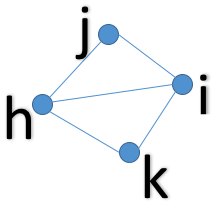
\includegraphics[width=.23\textwidth]{edge_patch2}
  \end{center}
  \caption{The edge patch $<h,i;j,k>$.}
\end{wrapfigure}
  
A \emph{framework} in the plane is a finite graph $G=(V,E)$ and a mapping $p: V \rightarrow \R^2$ such that there are no self-loops, ie. $p(a) \neq p(b)$ if $(a,b) \in E$ \cite{mccProof}. Essentially, a framework is a graph and its embedding.The notation for frameworks is as follows: 

\begin{itemize}
	\item The framework is written as $G(p)$
	\item $p(a)$ is a point treated as a position vector. 
	\item Joints are written as $p(i)$ or more commonly $p_i$.
	\item Bars are written as $p_ip_j$ or $\{i,j\}$
	\item Edges are written $ij$.
\end{itemize}

The forces exerted by a bar, an edge placed in the embedding, are a pair of equal but opposite forces along the bar: $\omega_{ij}(p_j - p_i)$ at $p_i$ and $\omega_{ij}(p_i - p_j)$ at $p_j$. If $\omega_{ij} \geq 0$ the force is a tension force, otherwise it is a compression force. The forces at a joint $p_i$ are at equilibrium if $\sum_j \omega_{ij}(p_j-p_i) = 0$\cite{mccProof}.

A \emph{self stress} on a framework $G(p)$ is an assignment of scalars $\omega_{ij}$ to the edges such that for each vertex $i : \sum_j \omega_{ij}(p_i - p_j) = 0$ \cite{mccProof}. This means the total force on each vertex is zero. 
\begin{itemize}
	\item A self stress is non-trivial if some $\omega_{ij} \neq 0$.
	\item A self stress is full if all $\omega_{ij} \neq 0$.
	\item A framework is independent if it supports only the trivial self stress with all scalars zero.
	\item The support is the set of edges on which $\omega_{ij} \neq 0$.
	\item The self stress is full if the support is the entire graph.
\end{itemize}

A \emph{combinatorial oriented polyhedron} is a finite set of vertices, faces and edge patches such that \cite{mccProof}:
\begin{enumerate}
	\item If $<h,i;j,k> \in E$ then $<i,h;k,j> \in E$ but $<h,i;k,j> \not\in E$ and $<h,i;j,k> \not\in E$. Essentially, there are two edge patches for each edge in the graph, notated as indicated.
	\item For each vertex $a_0$ all edge patches with first entry $a_0$ form a cycle $<a_0,i_s;j_s,k_s>$ for $1\leq s \leq t$, $t\geq3$ with $k_s = j_s + 1$ and $j_t = k_1$ where all $k_s$ and $i_s$ are distinct. 
	\item For each face $F^0$ all edge patches with last entry $F^0$ form a cycle $<h_s, i_s;j_s,F^0>$ for $1\leq s \leq t$ $t\geq3$ with $i_s = h_s + 1$ and $i_t = h_1$ where all $h_s$ and $j_s$ are distinct.
	\item Each pair $a_0$, $a_1$ is joined by a vertex edge path. Each pair of faces is connected by a face-edge path. 
\end{enumerate}

Lastly, two other definitions that will be references are as follows:
A \emph{cut} is a partition of the vertices of a graph into two disjoints subsets and an \emph{annulus} is a ring-shaped object bounded by two concentric circles. 

\subsubsection{Spherical Combinatorial Polyhedron}
A combinatorial polyhedron is spherical if every closed path of faces and distinct edges $<h_r,i_r;j_r,k_r>$ for $1 \leq r \leq t$ such that $j_{r+1} = k_r$ and $j_1 = k_t$ disconnects the vertices \cite{mccProof}. If so, then the dual is also spherical. 

A graph $G$ is a graph of a spherical combinatorial polyhedron if and only if its is vertex 2-connected and edge 3-connected \cite{mccProof}. Ie. the graph of a spherical polyhedron is planar.

\textsc{Proof}

Part A: First it must been shown that the graph is vertex 2-connected and edge 3-connected. From property two above, the graph is already known to be connected. We prove this by contradiction. First we assume the graph an be separated by removing an arbitrary vertex $v_0$. Next we select subgraph $C$ surrounded by an annulus in the sphere, reinserting $v_0$. We must insert wedges from $C$ to $v_0$, around $C$ this breaks the annulus into a single face contacting $v_0$ twice. This contradicts property 3 from above \cite{mccProof}.
To show the graph is edge 3-connected assume that removing 2 edges disconnects the graph. These two edges go from $\{a,a^{'}\}$ and $\{b, b^{'}\}$ joining 2 components. The two edges cut out two faces $F^1$ and $F^2$. In the cycle around $F^1$, the face $F^2$ now occurs across two edges. This contradicts property 3 of the combinatorial oriented polyhedron \cite{mccProof}.

Part B:
Given any vertex 2-connected, edge 3-connected graph, form a corresponding combinatorial spherical polyhedron: arcs and vertices surround simple disks which become faces along with the outer face. After placing point $f^j$ in each face we add $<h,i;j,k>$ if and only if the circuit $p_h, f^i,p_i,f^k$ around an arc $d_{ij}$ is clockwise. This means that the patches around each vertex form a cycle, and since the graph is not a multi-graph the vertices are distinct. If a cycle around a vertex contained a face twice, then the graph could be disconnected by removing this vertex. This contradicts the vertex 2-connectivity. Additionally, the patches around a face form a cycle. Assume a vertex occurs twice in a cycle. Since there are no loops removing it violates 2-connectivity. Assume an adjacent face in a cycle occurs twice, removing edges violates 3-connectivity \cite{mccProof}.

\subsection{Proof of Maxwell Cremona Theorem}
The following is a reproduction of the proof by Carpo and Whiteley \cite{mccProof}.
\subsubsection{Part 1: Stress and Reciprocal Diagram}
A reciprocal framework, or dual embedding, $H* = ((F,E);P)$ on the dual combinatorial polyhedron is a framework such that for each edge patch $<h,i;j,k>$  the vector $v_e = p_i - p_h$ is perpendicular to the vector $v^e = p^k - p^j$ from the reciprocal. \\
\\
\textsc{Theorem} A plane framework on a planar vertex 2-connected, edge 3-connected graph, supports a self stress if and only if it has a reciprocal framework. \\
\\
\textsc{Proof} Starting with a planar drawing of a graph, form the associated spherical polyhedron. 

A note on notation: $90^o$ clockwise rotation will be written $u^\bot$ and $90^o$ counter-clockwise rotation will be written $-u^\bot$

Part A: Assume the spherical polyhedron has a reciprocal framework.
For each edge patch $<h,i;j,k>$ we will use the equation $\omega_{hi}(p_i - p_h) = -(P^k - P^j)^\bot$ or $\omega_ev_e = (V^e)^\bot$ to define scalars $\omega_{hi} = \omega_e$. All scalars will not equal zero because $P^j \neq P^k$ in a framework. From the facial polyhedrons of the reciprocal framework we get $\sum\omega_ev_e = 0 = \sum\omega_{hi}(p_i - p_h)$.

Part B: Assume we have a full self stress on the framework.
Pick a face $F^0$ and a point $P^0$ for the this face. Any other face is connected by a simple face-edge path of edge patches $\{...e...\}$. We define $P^1 = P^0 + \sum\omega_ev_e^\bot$. This is a consistent definition provided that two different paths from $F^0$ to $F^1$ give the same point $P^1$. Two such paths form a closed path on the spherical polyhedron and therefore the edges of the path form a cut set for the graph of the polyhedron. If we travel on one path and back on the other we see the sums on the two paths are equal, as required $\sum\omega_ev_e = \sum\omega_e^{'}v_e^{'} = 0$ For each edge $e = <i,h;j,k>$ the path from $P^j$ to $P^k$ is this single edge and the difference in position is $P^j - P^k = -\omega_ev_e^\bot$. Thus, we have a true reciprocal.

Part B of this proof in layman's terms is that from the definition of a self stress, a simple cycle that sums around a vertex will equal zero. As a result of this fact, you can divide the graph into cut sets that each have a self stress of zero. Adding these self stresses up, you obtain the final result of zero.

These results generalize to any combinatorial oriented polyhedron. \\
\\
\textsc{Corollary} Given a combinatorial oriented polyhedron $(V,F,E)$ and any framework $H = ((V,E);P)$ there is a full self stress on the framework satisfying $\sum \omega_ev_e = 0$ if and only if there is a reciprocal framework $H* = ((F,E);P)$. 

\textsc{Proof} Part A: Given a reciprocal there is a full self stress.
For any face-edge cycle $\omega_e v_e = (V^e)^{\bot}$ since the vectors $V^e$ form a closed polygon in the reciprocal $\sum_e(V^e)^\bot = 0$.

Part B: Given a full self-stress $P^1 = P^0 + \sum_e \omega_ev_e^\bot = reciprocal$.
Given any two paths between $F^0$ and $F^1$ we get the same value for $P^1$ since the sum up one path and back the other is a cycle and yields zero.


\subsubsection{Part 2: Lifting and Reciprocal Diagrams}
\textsc{Definition} The \emph{vertex diagram} of an oriented polyhedral surface $((V,F;E);Q)$ is the plane framework on the projection with the graph $(V,E)$ and points $p_i = (x_i,y_i,0)$ if $q_i = (x_i,y_i,z_i)$.


\textsc{Definition} The \emph{face diagram} of an oriented polyhedral surface $((V,F;E);Q)$ is the framework with the graph $(F,E)$ and points $P^i = (A^i,B^i,0)$ for $F^i$ if $Q^i = (A^i,B^i,1,C^i)$. The points in the face diagram are the intersections of the plane $z=0$ with the normals to the faces through the point $(0,0,-1)$. Equivalently, they are the negatives of the gradients of the face planes threaded as functions of $x$ and $y$.
 
 \textsc{Definition} The \emph{Maxwell polarity} in the space is the pair of transformations $L$ and $L^{-1}$ between points in $R^3$, triples $(x,y,z)$, and non-vertical planes in $R^3$, quadruples $(A,B,1,C)$, defined by $L(x,y,z)=(x,y,1,z)$ and $L^{-1}(A,B,1,C) = (A,B,C)$.
 
 The Maxwell polarity preserves incidences: it takes a point $q$ on plane $Q$ to the plane $L(q)$ through the point if and only if the point lies on the Maxwell paraboloid $x^2 + y^2 + 2z = 0$.
 
 \textsc{Proof} Assume we have a point $q$ on a plane $Q$: $Ax + By + z + C = 0$. After transformation to $L(q)$ and $L^{-1}(Q)$ we have: $xA + yB + C + z = 0$, so the new plane contains the new point. If $q$ lies on $L(q)$ we have $x^2 + y^2 + z + z = 0$, and the point lies on the paraboloid. 
 
 Recalling that for an edge patch $e = <h,i;j,k>$, the turning moment is $m_e = p_j \times p_i$. In a similar manner, for the dual edge in the reciprocal we have $V^e = (P^k - P^j)$ and $M^e = P^k \times P^j = (P^k - P^j)\times P^j)$.
 
 \textsc{Theorem} Part A: For any polyhedral surface $((V,F;E);p)$ the vertex diagram and the face diagram are reciprocal frameworks.
 Part B: The dependencies induced by this reciprocal pair satisfy first, the vector condition $\sum \omega_e v_e = 0$ and the moment condition $\sum \omega_e m_e = 0$ and second, the dual conditions $\sum \omega^e V^e = 0$ and $\sum \omega^e M^e = 0$.
 
 \textsc{Proof} Part A: For each face $F^i$ the vector $N^j = (A^j, B^j,1)$ is normal to the plane $Q^j$. For each edge $e = <h,i;j,k>:  (x_h-x_i,,y_h-y_i, z_h-z_i)=(q_h-q_i) = \omega^e N^j \times N^k = \omega^e(B^j-B^k,A^k-A^j,A^jB^k-A^kB^j)$. This shows that $-\omega^e(A^j-A^k,B^j-B^k)^\bot = (x_h - x_i, y_h-y_i)$ or $-\omega^e(V^e)^\bot = v_e$. The frameworks are reciprocal, with scalars $\omega^e$ for the self stress in the face diagram.
 PartB: Around any vertex-edge cycle of the polyhedron, $\sum(x_h - x_i, y_h-y_i, z_h-z_i) = 0$ as a vector sum on the polyhedral surface. For any edge $(x_h-x_i,y_h-y_i) = -\omega^e(A^j-A^k,B^j-B^k)^\bot = -\omega^e(V^e)^\bot$. Therefore, for any vertex-edge cycle in the original polyhedron, $\sum_e \omega^eV^e = \sum_e \omega^e(x_h-x_i,y_h-y_i)^\bot = 0$. In addition $(z_h-z_i) = \omega^e(A^jB^k-A^kB^j) = -\omega^e(P^j-P^k) \times P^j = \omega^eM^e$. Therefore, for any vertex-edge cycle in the original polyhedron $\sum \omega^eM^e = \sum(z_h-z_i) = 0$. 
 
 We still must show that $\sum \omega_e v_e = 0$ and that $\sum \omega_em_e = 0$ for any face-edge cycle in the vertex diagram. We apply the Maxwell polarity. This makes the vertex diagram of the original polyhedral surface into the face diagram of the polar polyhedral surface. As a face diagram it must satisfy $\sum \omega_e v_e = 0$ and $\sum \omega_em_e = 0$.
 
 \textsc{Theorem} Given a reciprocal pair of plane frameworks $H=((V;E);p)$ and $H^* = ((F;E);P)$ on the oriented combinatorial polyhedron $(V,F;E)$ the following are equivalent: 
 \begin{enumerate} 
 	\item The reciprocal dependence in the original framework satisfies $\sum \omega_em_e = 0$ and second, there is a polyhedral surface 
 	\item There is a polyhedral surface $((V,F;E);Q)$ with $H$ as its vertical projection and $H^*$ as its face diagram.
	\item There is a polar polyhedral surface $((F,V;E);Q^*)$ with $H^*$ as its vertical projection and $H$ as its face diagram.
	\item The dependence in the reciprocal framework satisfies the equation: $\sum \omega^eM^e = 0$
\end{enumerate}
\textsc{Proof} We know that (ii) $\Rightarrow$ (iv) by the previous theorem. 

(iv) $\Rightarrow$ (ii): Choose a vertex $p_0$ adn set $q_0 = (x_0, y_0,0)$. For each face $P^j$ we define $N^j = (A^j,B^j,1)$, which will become its normal. We recall that $\omega^eN^j \times N^k = \omega^e(B^j-B^k,A^k-A^j, A^jB^k-A^kB^j) = (V^e) + (0,0,M^e)$. For every other point $p_1$ there is a vertex-edge path from $v_0$ to $v_1$, We use this path to set: $q_1 = q_0 + (\sum \omega^eN^j \times N^k) = (x_0,y_0,0) + (\sum \omega^eV^e + (0,0,\omega^eM^e)) = (x_0,y_0,0) + \sum \omega^eV^e + \sum \omega^eM^e = (x_1,y_1,0) + (0,0,\sum \omega_eM^e)$. Since $\sum{e}\omega^eM^e = 0$ on any vertex-edge cycle, $z_1$ is well defined.

(ii) $\Leftrightarrow$ (iii). This equivalence follows from an application of the Maxwell polarity to the given polyhedral surfaces.

(ii) $\Leftrightarrow$ (i). This is the dual of (ii) $\Leftrightarrow$ (iii), and follows by the same argument. 

 
 
\subsubsection{Result}

Given a planar framework with an associated combinatorial spherical polyhedron $(V,F;E)$ the following are equivalent:
\begin{enumerate}
	\item There is a self stress on the framework with all $\omega_e \neq 0$.
	\item There is a reciprocal framework on the dual graph $(F;E)$.
	\item There is a spatial polyhedron $((V,F;E);Q)$ with the framework as its vertical projection (and the reciprocal as its face diagram).
 \end{enumerate}
 
 Combining this result with Tutte's algorithm and the knowledge that if the fixed outer face in Tutte's algorithm is a triangle, negative weights can be assigned to get a global equilibrium stress almost yields a proof of another theorem known as Steinitz's Theorem. However, if the outer face of the embedding is not a triangle, the dual embedding will have a triangular outer face. This can be remedied with the knowledge that, for every 3-connected planar graph, $G$, either $G$ or its dual has a triangle. Therefore, using the dual graph an equilibrium stress can be obtained. After this, using the Maxwel Cremona Theorem a polytope can be obtained. This is a path that has been used to prove Steinitz's theorem in the past. Though we will not reproduce this proof, we state the result. 
 
 \textbf{Steinitz's Theorem}: Every planar 3-connected graph can be represented by a convex 3-dimensional polytope \cite{realizationSpaces}.
 
 In total this means that every Circle packing can be represented by a Delaunay Triangulation (embedding with an equilibrium stress), which has multiple equivalent representations including, a convex 3-dimensional polytope (lifting) and a reciprocal diagram (dual embedding or Voronoi Diagram). 

This also yields intuition for a Circle packing algorithm which, though has not been proven to always work, seems to work very well on small problem instances. This algorithm is a force-directed algorithm which computes the embedding of the graph by using Tutte's algorithm to iteratively modify the force of each edge by changing the distance between the two points and updates the radii of each circle iteratively. The algorithm is as follows: While the embedding is not a valid Circle Packing, for every edge, reposition the two vertices it connects, provided they are interior vertices, based on the stress of the edge. Then, for every edge, calculate the length of the edge and determine if the radii of the two circles add up to that distance. If not, increase the stress and the radii, otherwise, decrease the stress and the radii. This algorithm can be observed working in our application.
 
\section{Stereographic Mappings}
There are many equivalent representations of Circle Packings in two dimensions, namely, Weighted Delaunay Triangulations, dual circle packings, and Voronoi diagrams. Additionally, from the Maxwell Cremona theorem Circle packings can be represented as convex 3-dimensional polytopes, essentially they can be lifted into three dimensional space. However, this is not the only way to represent a Circle packing in three dimensions. Using Stereographic Mappings, an additional representation can be discovered. 

Circle packings can also be represented on the Riemann sphere. In this section, we will cover circle packings on the sphere and the insights this representation yields.

\subsection{Riemann Sphere}
The euclidean plane that we have discussed thus far can be represented mathematically by: $\R^2 = \C = \{z = x + iy : x, y \in \R \}$. In contrast, the Riemann sphere, also known as the unit sphere or the complex projective line is modeled as such: $\mathbb{P} = \{(x,y,z):x^2 + y^2 + z^2 = 1\} \subset \R^3$. This sphere can be thought of as the wrapping of the complex plane around a ball, with the addition of one point at infinity. The plane is found to be a subset of the sphere via stereographic projection, which is a mapping that projects a sphere onto the plane. This mapping is bijective and is often used to describe the mapping of the plane to the sphere as well. Formally, starting at the infinity point, which for simplification we will place at the north pole, drawing a line towards a point on the plane, let the point where the line punctures the sphere be $p = (x,y,z)$ and the point where it touches the plane point $w = u + iv$. Then using similarity of triangles and recalling that $x^2 + y^2 + z^2 = 1$ the following relationships can be obtained: $u = \frac{x}{1 + z}$, $v = \frac{y}{1+ z}$. $z = \frac{1 = (u^2 + v^2}{1 + (u^2 + v^2)}$, $x = u(1+z)$, and $y =v(1+z)$.

Circle packings can be mapped onto this sphere via stereographic projection to obtain an essentially unique circle packing. This is a result of the \textbf{Koebe-Andreev-Thurston Theorem} which says the following \cite{stephenson05introduction}:

\textsc{Theorem}: Let $K$ be a combinatorial sphere. Then there exists an essentially unique univalent circle packing $P_K$ for $K$ on the Riemann sphere $\mathbb{P}$.

These packings are unique up to M\"{o}bius Transformations.

\begin{figure}[h]%
    \centering
    \subfloat[User input]{{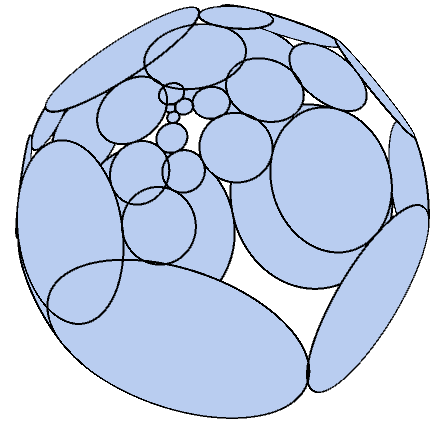
\includegraphics[width=.4\textwidth]{riemannsphere} }}%
    \qquad
    \subfloat[User input packed]{{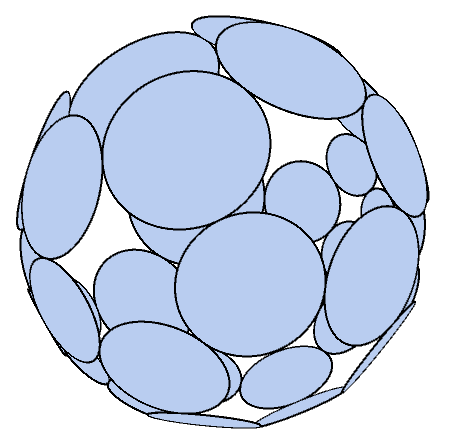
\includegraphics[width=.4\textwidth]{riemannsphere_packed} }}%
    \caption{Stereographic projection onto the Riemann Sphere}%
    \label{fig:riemann}%
\end{figure}

\subsection{M\"{o}bius Transformations}
 A \textbf{M\"{o}bius Transformation} of a plane can be obtained by performing the stereographic projection of the plane onto a sphere, then rotating or moving the sphere and then performing the stereographic projection back onto the plane. 
  Formally, a M\"{o}bius Transformation is a rational function defined on the extended complex plane $\CP = \C\cup\{\infty\}$ of the form:
  \begin{equation} 
  	f(z) = \frac{az+b}{cz+d}
  \end{equation}
  where $z\in\CP$ is a complex variable and $a,b,c,d\in\CP$ are complex numbers such that $ad - bc$ $\neq$ $0$ \cite{stephenson05introduction}. These transformations are invertible and if performed on circle packings, transform circle packings to equivalent circle packings without losing any information. Therefore, circle packings in the plane are unique up to M\"{o}bius Transformations. In our application, M\"{o}bius Transformations can be performed from both the spherical and planar view by moving the mouse to rotate the sphere or transform the plane.
    \begin{figure}[h]%
	\centering
	\subfloat[A circle packing.]{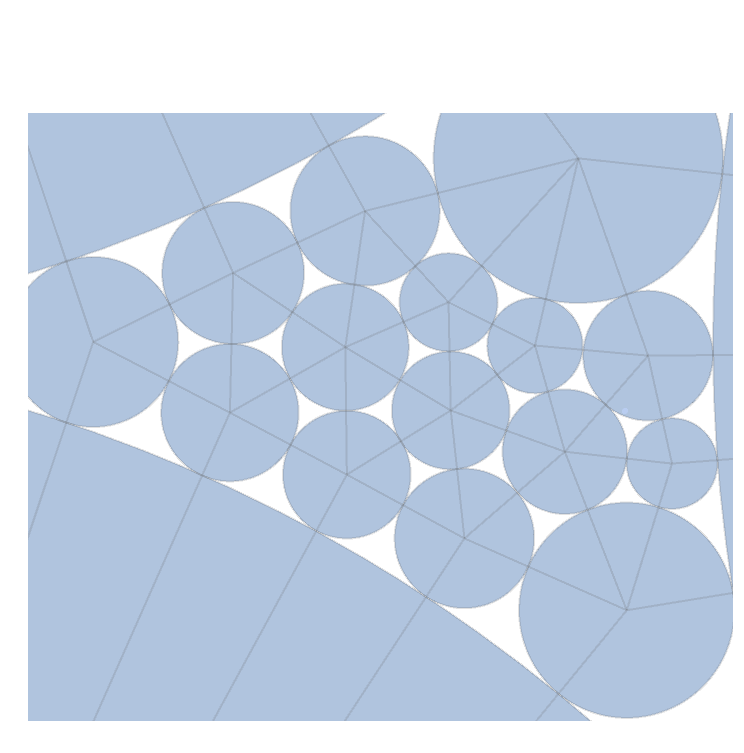
\includegraphics[width=.35\textwidth]{input_packedcropped}}%
	\qquad
	\subfloat[A M\"{o}bius Transformation of the packing in (a).]{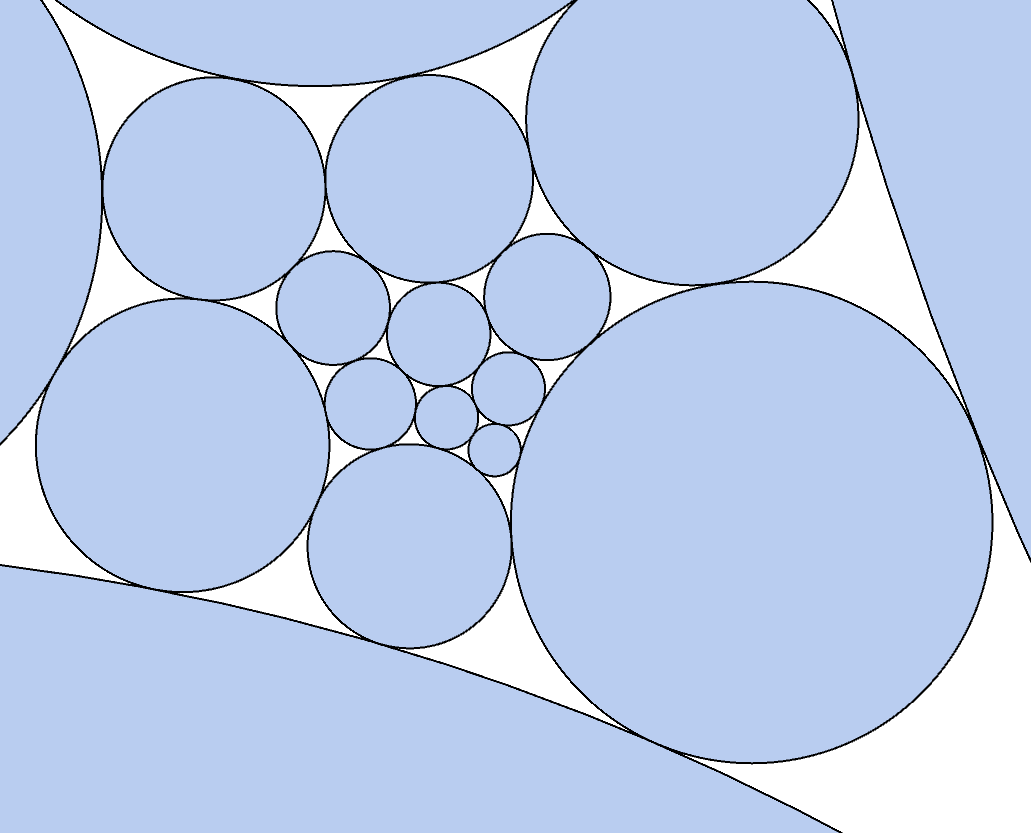
\includegraphics[width=.35\textwidth]{packing_transformed}}%
	\caption{M\"{o}bius Transformations in the plane.}%
	\label{fig:mobiusplane}%
\end{figure}

\begin{figure}[H]%
	\centering
	\subfloat[A Circle Packing on the sphere.]{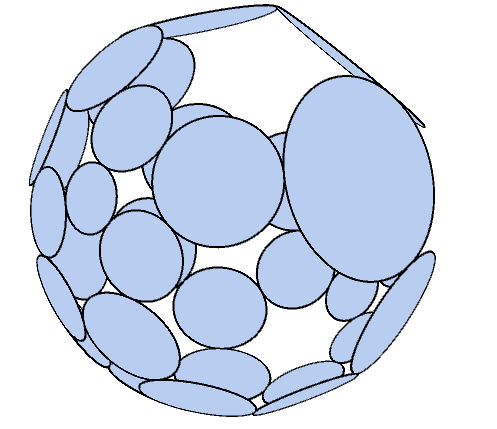
\includegraphics[width=.35\textwidth]{sphere1}}%
	\qquad
	\subfloat[A M\"{o}bius Transformation of the packing in (a).]{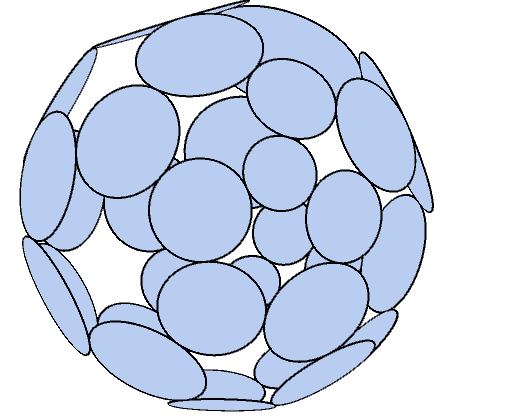
\includegraphics[width=.35\textwidth]{sphere2}}%
	\caption[]{M\"{o}bius Transformations on the Riemann Sphere.}%
	\label{fig:mobiussphere}%
\end{figure}

\section{Conclusion}
Circle Packings have many equivalent representations that can be exploited to develop new algorithms to both make better packings and obtain them more quickly. These representations include Delaunay Triangulations, Voronoi Diagrams, Parabolic Liftings, Koebe Polyhedrons, and Packings on the Riemann Sphere. Through examining one of these representations, the Delaunay Triangulation, and its properties as observed by Tutte and Maxwell, a new algorithm for computing Circle Packings based on equilibrium forces was developed. In the future, a combination of these representations could be used to develop a new non-linear optimization algorithm based on optimizing different aspects of each equivalent representation.

\bibliographystyle{plain}
\bibliography{references}
\end{document}  